\documentclass[letterpaper,12pt]{article}
\usepackage{subfiles,amsmath,amssymb,float,epstopdf}
\numberwithin{equation}{subsection}
\bibliographystyle{plain}
\usepackage[margin=1.0in]{geometry}
\usepackage[hypcap]{caption}
\usepackage{subcaption}
\usepackage{hyperref}
\usepackage{indentfirst}
\usepackage{graphicx}
\usepackage{setspace}
\doublespacing
\graphicspath{ {./img/} }

\begin{document}

\title{\textbf{Molecular Dynamics}}
\author{Gregorio Ponti,\\
	Agust{\'in} I{\~n}iguez\\
	Physics 480, \\
	Computational Physics,\\
	Spring 2015\\
	Michigan State University, \\
	Delft University of Technology}
\maketitle

\newpage
\tableofcontents

\newpage
\section{Introduction}
Many-body systems have been a problem in physics as it is hard to determine quantities over the whole system. In statistical mechanics, computations can be done over the average of the system but it requires to know many variables of the system. An advantageous way to determine such quantities is using computer simulations. Two methods have been developed to do so: molecular dynamics and Monte Carlo methods. In this investigation, molecular dynamics will be used to look at an N-body system and determine several physical quantities for the system. Systems are simulated classically as atoms or molecules and placed into a potential and allowed to interact for a period of time. Molecular dynamics has the advantage of providing a method to determine expectation values of statistical quantities as well as dynamical phenomena$ ^{\cite{JM}}$.
\subsection{FCC}
\indent The simulation created will look at Argon atoms interacting in a potential created by all the surrounding atoms and placed in a cube to interact. The atoms are placed in a Bravais Face-Centered Cubic (FCC) lattice. This is chosen because this is the ground state configuration of noble gases, like Argon. The FCC lattice is a simple cubic lattice (atom at each of the vertices) with an additional point on the center of each square face$ ^{\cite{A&M}}$. A simple diagram for an FCC lattice can be seen in Figure \ref{fig:FCC}.
\begin{figure}[H]
        \centering
        \caption{Points on a face-centered cubic Bravais lattice \label{fig:FCC}}
    %    \begin{subfigure}[b]{\textwidth}
                \centering
                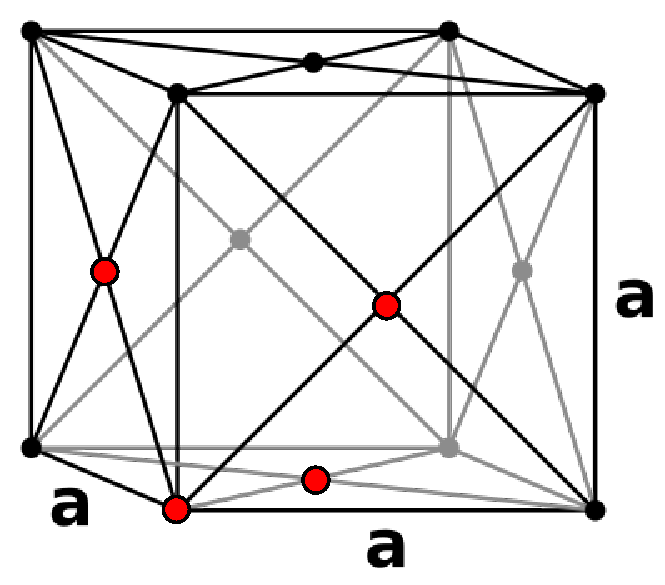
\includegraphics[width=0.75\textwidth]{fcc.png}
    %    \end{subfigure}
\end{figure}
Let's say that the length of one side is $a$. Then the distance from an atom to it's nearest neighbour is given by $a/ \sqrt{2}$. This will be of use when initializing the system and the positions of the particles.
\subsection{Lennard-Jones Potential}
When looking at the interactions between the individual particles, the most convenient from is by using the Lennard-Jones potential. This potential is given by
\begin{equation}
U(r) = 4 \epsilon \left[ \left( \frac{\sigma}{r}\right)^{12} - \left( \frac{\sigma}{r}\right)^{6}\right]
\end{equation}
where $\epsilon$ and $\sigma$ are visualized in Figure \ref{fig:LJP}
\begin{figure}[H]
        \centering
        \caption{Diagram of the Lennard-Jones Potential \label{fig:LJP}}
    %    \begin{subfigure}[b]{\textwidth}
                \centering
                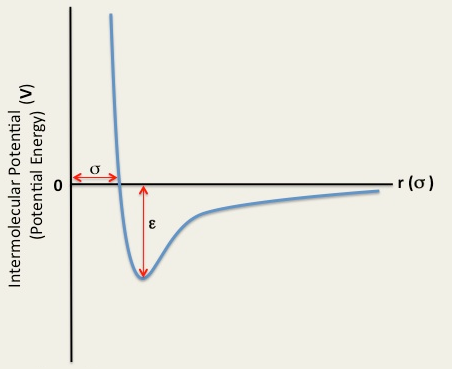
\includegraphics[width=0.75\textwidth]{LJP.png}
    %    \end{subfigure}
\end{figure}
The reason that the Lennard-Jones potential is used is because it calculates the potential for pairs of particles which is useful for molecular dynamics. This will allow the system to be dependent on the sum of all potentials from all particles, something that is very difficult to do without a computer but computationally very inexpensive.

\newpage
\section{Methods}
\subsection{Initialization}
The first problem to solve is that of the initialization of the system. This takes two things to be set up: the position of the atoms (FCC lattice) and the initial velocity of the atoms. \\
\indent For the position of the atoms, the minimum distance between particles was found using the potential. The result of this was a minimum distance of $2^{1/6}$. From this, it was calculated that the length of each side of the unit cube is $2^{2/3}$. This is assuming that $ \sigma = 1$ to simplify the calculation. Also, $\epsilon$ is set to 1 for the same reasons. In terms of the method of initialization, as opposed to going particle by particle and assigning a set of coordinates to it, the reverse was done. The positions of each point of the FCC lattice was found and then assigned to the next particle in line. The reason this was done is that the determination of the position as reference to the previous position is easier to calculate and iterate over than the iteration of the position dependent on the number of the particle that is placed. \\
\indent For the velocity, a Gaussian distribution of the velocities was created, centered around 0. To do this, two random values between 0 and 1 are obtained. The first value is then placed in between the range of the Gaussian distribution ($ -3T/2$ to $3T/2$) and it's probability is determined using
\begin{equation}
P = \frac{1}{\sqrt{2.0 \cdot T \cdot \pi}} e ^{\frac{-x^{2}}{2.0 \cdot T}}
\end{equation}
This probability is then checked against the second random value. If the probability is greater than the second random number, then the value for the first random value is kept. If not, the value is discarded and the process is repeated until a value is kept. The first random value is then kept as the velocity. \\
\indent To make sure that the system is in the center-of-momentum frame ($\Sigma v = 0$), the velocities for all the particles are added up and the sum should equal 0. If not, then the remaining value is divided by the number of particles and then added to each velocity.
\subsection{Time Evolution}
The time evolution is split into two main components: the Verlet algorithm and the thermostat. The Verlet algorithm is used to move the particles and change the velocity in a leapfrog mechanism$^{\cite{Verlet}}$ while the thermostat maintains the temperature at a fixed value. \\
\indent The Verlet algorithm has a total of three steps. The first updates the velocity at the first half time step.
\begin{equation}
\textbf{v'}(t) = \textbf{v}(t) + \textbf{F}(t) \cdot \frac{\Delta \textbf{t}}{2}
\end{equation}
The second step is to update the position using
\begin{equation}
\textbf{r}(t + \Delta t) = \textbf{r}(t) + \Delta \textbf{t} \cdot \textbf{v'}(t)
\end{equation}
When the position is updated, there is a check to see if the particle passed the boundary. If this is true the particle is placed on the other side by adding/subtracting the length of the system from the updated position. Finally the velocity is updated
\begin{equation}
\textbf{v}(t + \Delta t) = \textbf{v'}(t) + \textbf{F}(t + \Delta t) \cdot \frac{\Delta \textbf{t}}{2}
\end{equation}
\indent To keep the temperature constant, a function thermostat is defined. The purpose of this function is to increase or decrease the velocities based on the calculated temperature of the system compared to the desired. This is easily constructed as the ratio is given by
\begin{equation} \label{eq:ratio}
\gamma = \sqrt{\frac{3(N-1) T_{target}}{(\Sigma v)^{2}}}
\end{equation}
Once this ratio is found, the existing values of velocity are multiplied by $\gamma$ to put the system at the desired temperature. This is applied over a certain amount of time steps because after a certain point, the system stabilizes and the temperature stays constant.
\subsection{Physical Quantities}
The physical quantities determined from the system are all from statistical mechanics. The energies of the system (kinetic, potential and total) are all easy to determine from the velocities and the Lennard-Jones potential. Also easily determined is the temperature of the system at each time step. The more complex physical quantities found in this simulation were the pair correlation function and the pressure of the system. Both of these values depends on the distances between all the pairs of the system. \\
\indent First off, the energies are easily calculated. The kinetic energy of the system is given by
\begin{equation}
KE = \dfrac{1}{2} m \cdot \Sigma (v^{2})
\end{equation}
and the potential energy of the system by the Lennard-Jones Potential. The total energy of the system is a sum of the two. For the temperature, two ways can be used to determine the temperature at each time step. The first is to use the kinetic energy found. The second uses the velocity, found in Equation \ref{eq:temp}
\begin{equation} \label{eq:temp}
T = \dfrac{1}{3} m v_{rms} ^{2}
\end{equation}
\indent The pair correlation function gives a representation of the density of the system based on the distance between two particles. Consecutive circles are drawn around a reference particle and then rings of thickness $\Delta r$ are taken to find the distance between the reference particle and all other particles of the system (see Figure \ref{fig:PCF} for reference). When a particle is found in a ring, that particle is added to a bin that encompasses all the particles within that distance to the reference particle. This creates a histogram of the distances of the particles from one another. The expression for the pair correlation function is given by Equation \ref{eq:PCF}
\begin{equation} \label{eq:PCF}
g(r) = \dfrac{2V}{N(N-1} \dfrac{<n(r)>}{4 \pi r^2 \Delta r}
\end{equation}
\begin{figure}[H]
        \centering
        \caption{Diagram of the Pair Correlation Function \label{fig:PCF}}
    %    \begin{subfigure}[b]{\textwidth}
                \centering
                \includegraphics[width=0.50\textwidth]{pair_correl_example.png}
    %    \end{subfigure}
\end{figure}

\indent Finally, the pressure can be calculated. Using the virial equation
\begin{equation}
\sum_{i,j} r_{ij} F(r_{ij})
\end{equation}
the pressure can be calculated using equation \ref{eq:pressure}
\begin{equation}
\label{eq:pressure}
P = \frac{1}{V}(NT - \dfrac{\sum_{i,j} r_{ij} F(r_{ij})}{3}
\end{equation}

\newpage
\section{Results}
\subsection{Energy}
\begin{figure}[h!]
        \centering
        \begin{subfigure}[b]{0.4\textwidth}
                \centering
                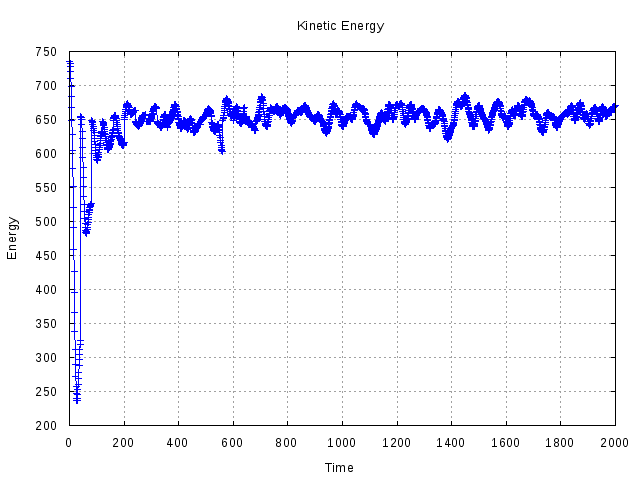
\includegraphics[width=5cm]{ener_kin.png}
        \end{subfigure}
        \quad
        \begin{subfigure}[b]{0.4\textwidth}
                \centering
                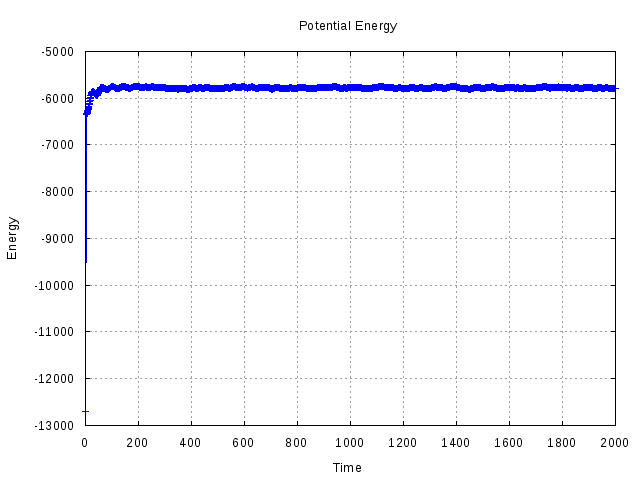
\includegraphics[width=5cm]{ener_pot.png}
        \end{subfigure}
	\end{figure}
\begin{figure}[H]
    %    \begin{subfigure}[b]{\textwidth}
                \centering
                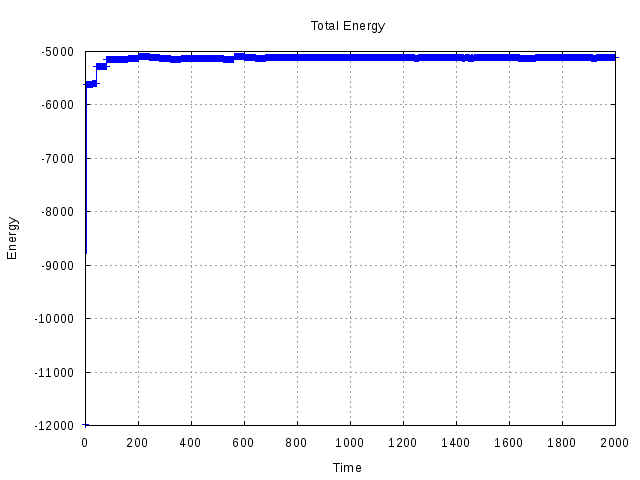
\includegraphics[width=0.75\textwidth]{ener_tot.png}
    %    \end{subfigure}
\end{figure}
\subsection{Temperature}
\begin{figure}[H]
    %    \begin{subfigure}[b]{\textwidth}
                \centering
                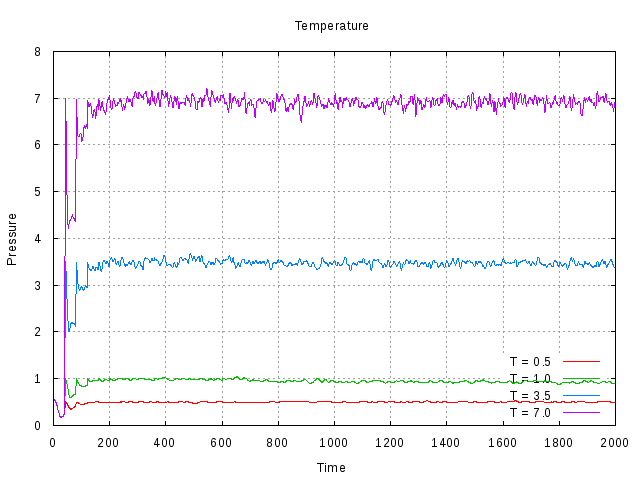
\includegraphics[width=0.75\textwidth]{temp.png}
    %    \end{subfigure}
\end{figure}
\subsection{Pair Correlation}
\begin{figure}[H]
    %    \begin{subfigure}[b]{\textwidth}
                \centering
                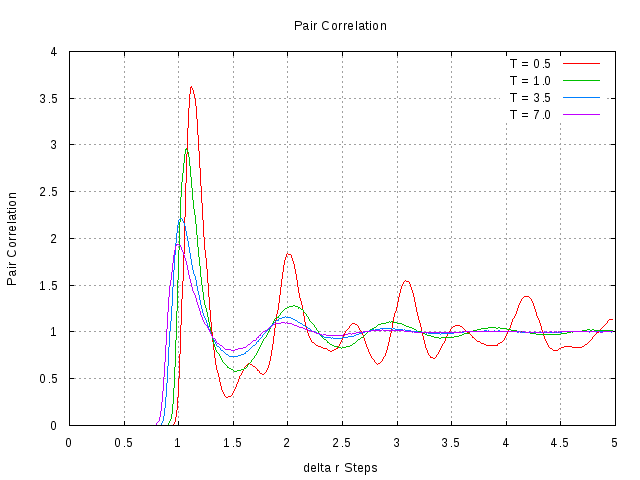
\includegraphics[width=0.75\textwidth]{pair_corre.png}
    %    \end{subfigure}
\end{figure}
\subsection{Pressure}
\begin{figure}[H]
    %    \begin{subfigure}[b]{\textwidth}
                \centering
                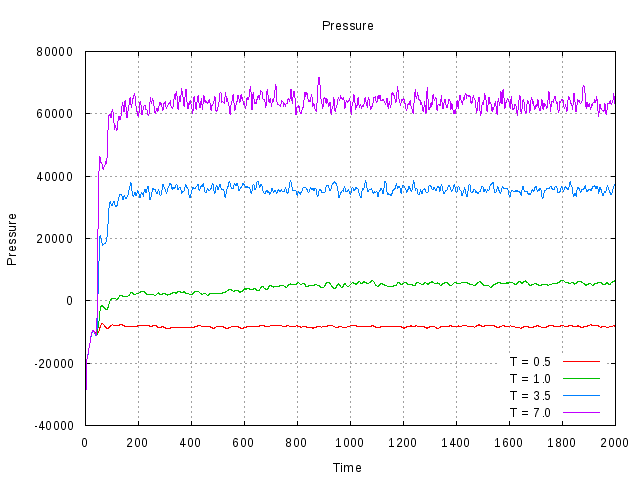
\includegraphics[width=0.75\textwidth]{pressure.png}
    %    \end{subfigure}
\end{figure}

\newpage
\thispagestyle{empty}
\mbox{}

\newpage
\section{References}
\begin{thebibliography}{99}
\bibitem{A&M} Ashcroft, N. W. and Mermin, N. D. \textit{Solid State Physics}. Thomson Learning, Inc. 1976. Print.
\bibitem{JM} Thijssen, J. M. \textit{Computational Physics}. Ch. 8. Cambridge University Press. 1999. Print.
\bibitem{Verlet} William C. Swope, Hans C. Andersen, Peter H. Berens, and Kent R. Wilson. \textit{A computer simulation method for the calculation of equilibrium constants for the formation of physical clusters of molecules: Application to small water clusters}. The Journal of Chemical Physics 76, 637 (1982); doi: 10.1063/1.442716
\end{thebibliography}

\end{document}
